\documentclass{article}
\usepackage{tikz}
\usetikzlibrary{arrows.meta,positioning,calc,shapes.geometric}
\pagestyle{empty}
\begin{document}
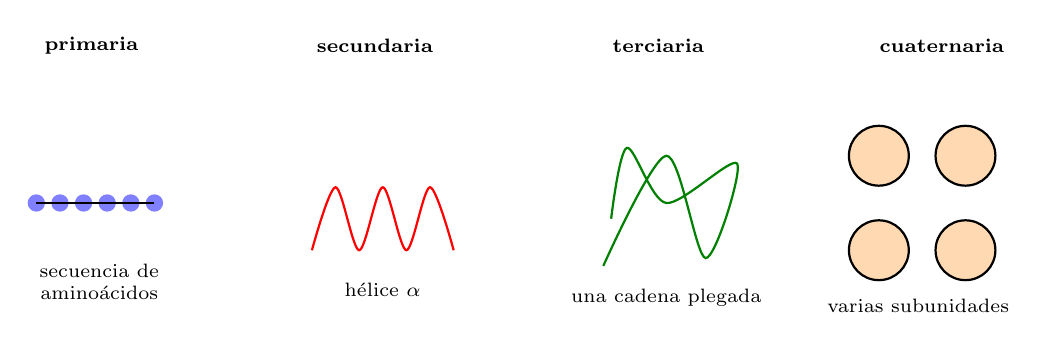
\begin{tikzpicture}
\tikzset{every node/.append style={align=center}}

\foreach \x/\t in {0/primaria, 3.6/secundaria, 7.2/terciaria, 10.8/cuaternaria} {\node[font=\bfseries\scriptsize] at (\x+0.9,3.2) {\t};}
\foreach \i in {0,1,2,3,4,5} {\fill[blue!50] (0.2+\i*0.3,1.2) circle (0.11);} \draw[thick] (0.2,1.2) -- (1.7,1.2);
\draw[thick, red] plot[smooth] coordinates {(3.7,0.6) (4.0,1.4) (4.3,0.6) (4.6,1.4) (4.9,0.6) (5.2,1.4) (5.5,0.6)};
\draw[thick, green!50!black] plot[smooth] coordinates {(7.4,0.4) (8.2,1.8) (8.7,0.5) (9.1,1.7) (8.2,1.2) (7.7,1.9) (7.5,1.0)};
\foreach \x/\y in {10.9/0.6, 12.0/0.6, 10.9/1.8, 12.0/1.8} {\draw[thick, fill=orange!30] (\x,\y) circle (0.38);}
\node[font=\scriptsize, align=center] at (1,0.2) {secuencia de\\ aminoácidos}; \node[font=\scriptsize, align=center] at (4.6,0.1) {hélice $\alpha$}; \node[font=\scriptsize, align=center] at (8.2,0.0) {una cadena plegada}; \node[font=\scriptsize, align=center] at (11.4,-0.1) {varias subunidades};

\end{tikzpicture}
\end{document}
